%\input{rus}
%\input{packages}
%\input{preamble}
%\input{listmain}
%\usepackage{amsmath}
%\usepackage{algorithm}
%\usepackage[noend]{algpseudocode}
%\makeatletter
%\def\BState{\State\hskip-\ALG@thistlm}
%\makeatother
%\algnewcommand\algorithmicforeach{\textbf{для всех}}
%\algdef{S}[FOR]{ForEach}[1]{\algorithmicforeach\ #1\ \algorithmicdo}

% I need packages above to succesfully compile tex file (Aleksandrov Nikita)

\begin{document}
\section{Критерии качества кластеризации}

Давайте детально разберем основные метрики, используемые для оценки качества кластеризации данных.  

Выбор подходящей метрики напрямую зависит от наличия или отсутствия предварительной разметки данных и от того, задано ли количество кластеров априори или оно подбирается в процессе кластеризации.

\subsection{Критерии, не требующие разметки выборки}

\subsubsection{Среднее внутрикластерное расстояние} \hfill\\

Название этой метрики говорит само за себя: она отражает среднее расстояние между всеми парами точек внутри одного кластера.  Иными словами, мы подсчитываем сумму расстояний между всеми парами точек в каждом кластере и делим на общее количество таких пар.  

Формула метрики выглядит так:
\begin{equation*}
     F_0 = \cfrac{\displaystyle\sum_{i=1}^n \sum_{j=i}^n \rho(x_i,  x_j) I[a(  x_i)=a(x_j)]}{\displaystyle\sum_{i=1}^n \sum _ {j=i}^n I[ a(x_i)=a(x_j)]}.
\end{equation*}

В формуле учитываются и пары вида $(x_i, x_i)$, что позволяет избежать неопределенности $\frac{0}{0}$ в случае, если кластер состоит всего из одной точки.  Однако, иногда для упрощения вычислений суммирование ведется только по парам $(x_i, x_j)$, где $i < j$, при этом для случая одноточечных кластеров значение метрики полагается равным нулю.

Вычисление этого критерия достаточно трудоёмко, поэтому можно также ввести средний квадрат внутрикластерного расстояния, если нам известные представители, или центры масс, кластеров $\mu_k$:
\begin{equation*}
     \Phi_0 = \displaystyle\frac{1}{nK} \sum_{k=1}^K \sum_{i=1}^n \rho(\mu_k,  x_i)^2 I[a(x_i)=k].
\end{equation*}

Наша цель при кластеризации -- получить максимально компактные кластеры, поэтому мы стремимся минимизировать значение этой метрики.  Чем меньше среднее внутрикластерное расстояние, тем лучше.

\subsubsection{Среднее межкластерное расстояние} \hfill\\

В отличие от предыдущей метрики, среднее межкластерное расстояние оценивает среднее расстояние между точками из разных кластеров.  

Формула выглядит следующим образом:
\begin{equation*}
     F_1 = \cfrac{\displaystyle\sum_{i=1}^n \sum_{j=i}^n \rho(x_i,  x_j) I[a(  x_i)\ne a(x_j)]}{\displaystyle\sum_{i=1}^n \sum _ {j=i}^n I[ a(x_i)\ne a(x_j)]}.
\end{equation*}

Здесь, наоборот, мы стремимся к максимизации этого значения.  Чем больше расстояние между кластерами, тем лучше разделение.  

\subsection{Критерии, требующие разметки выборки}

Следующие метрики требуют, чтобы мы заранее знали, к какому классу принадлежит каждый объект в наборе данных.  Это позволяет сравнить результаты кластеризации с истинным распределением данных.

Мы будем обозначать кластеры, полученные в результате кластеризации, как $k \in \{1, \ldots, K\}$, а истинные классы -- как $c \in \{1, \ldots, C\}$.

\subsubsection{Гомогенность} \hfill\\

Если у нас есть разметка, то можно свести задачу кластеризации к использованию методов классификации. Если размеченных данных достаточно много, то обучение классификатора -- более подходящий подход. Однако часто возникает ситуация, когда данных достаточно для оценки качества кластеризации, но всё ещё не хватает для использования методов обучения с учителем.

Пусть $n$ -- общее количество объектов в выборке, $n_k$ -- количество объектов в кластере номер $k$, $m_c$ -- количество объектов в классе номер $c$, а $n_{c,k}$ количество объектов из класса $c$ в кластере $k$. Рассмотрим следующие величины:
\begin{gather*}
    H_{class} = -\displaystyle\sum_{c=1}^C \cfrac{m_c}{n} \log\cfrac{m_c}{n}, \\
    H_{clust} = -\displaystyle\sum_{k=1}^K \cfrac{n_k}{n} \log\cfrac{n_k}{n}, \\
    H_{class \vert clust} = -\displaystyle\sum_{c=1}^C \sum_{k=1}^K \cfrac{n_{c,k}}{n} \log\cfrac{n_{c,k}}{n_k}.
\end{gather*}

Несложно заметить, что эти величины соответствуют формуле энтропии и условной энтропии для мультиномиальных распределений $\cfrac{m_c}{n}, \cfrac{n_k}{n}, \cfrac{n_{c,k}}{n_k}$ соответственно.

Гомогенность кластеризации определяется такой формулой:
\begin{equation*}
    Homogeneity = 1 - \cfrac{H_{class \vert clust}}{H_{class}}.
\end{equation*}

Отношение $\cfrac{H_{class \vert clust}}{H_{class}}$ показывает, насколько уменьшается неопределенность в распределении классов (измеряемая энтропией), если мы знаем, к какому кластеру относится каждый объект. 

Худший сценарий -- когда отношение равно единице, то есть знание о кластерной принадлежности никак не помогает определить истинный класс объекта (энтропия не изменилась). 

Лучший случай -- когда каждый кластер содержит только объекты одного класса, и, следовательно, зная номер кластера, мы точно знаем истинный класс (гомогенность равна 1). Заметим, что тривиальный (и бессмысленный) способ добиться максимальной гомогенности -- это выделить каждый объект в отдельный кластер.

\subsubsection{Полнота} \hfill\\

Метрика полноты аналогична гомогенности, но использует условную энтропию $H_{clust \vert class}$, которая симметрична $H_{class \vert clust}$:
\begin{equation*}
    Completeness = 1 - \cfrac{H_{clust \vert class}}{H_{clust}}.
\end{equation*}

Полнота равна единице, когда все объекты, принадлежащие одному и тому же истинному классу, находятся в одном и том же кластере.

Тривиальный, но непрактичный способ получить максимальную полноту -- это объединить все объекты выборки в один большой кластер.

\subsubsection{V-мера} \hfill\\

Метрики гомогенности и полноты в кластеризации аналогичны точности и полноте в классификации.  V-мера, в свою очередь, аналогична F-мере и представляет собой гармоническое среднее гомогенности и полноты. Пусть $\beta$ - весовой параметр, тогда формула выглядит следующим образом:
\begin{equation*}
    V_\beta = \cfrac{(1+\beta) \cdot Homogeneity \cdot Completeness}{\beta \cdot Homogeneity + Completeness}.
\end{equation*}

В случае $\beta = 1$ получаем, что $V_1$-мера является просто средним гармоническим гомогенности и полноты:
\begin{equation*}
    V_\beta = \cfrac{2 \cdot Homogeneity \cdot Completeness}{Homogeneity + Completeness}.
\end{equation*}

Использование V-меры позволяет избежать тривиальных решений, таких как присвоение каждого объекта в отдельный кластер (максимальная гомогенность) или объединение всех объектов в один кластер (максимальная полнота).  V-мера обеспечивает сбалансированную оценку качества кластеризации, учитывая как гомогенность, так и полноту.

\subsubsection{Коэффициент силуэта} \hfill\\

Коэффициент силуэта — метрика качества кластеризации, не требующая наличия меток классов. Сначала он вычисляется для каждого объекта, а затем итоговая метрика для всей выборки определяется как среднее значение коэффициентов силуэта всех объектов.

Для вычисления коэффициента силуэта $S(x_i)$ нужны две величины:

\begin{itemize}
    \item $A(x_i)$ — среднее расстояние от объекта $x_i$ до всех других объектов в том же кластере.
    \item $B(x_i)$ — среднее расстояние от объекта $x_i$ до объектов ближайшего соседнего кластера.
\end{itemize}

Сам коэффициент силуэта вычисляется по формуле:
\begin{equation*}
    S(x_i) = \cfrac{B(x_i)-A(x_i)}{\max (B(x_i), A(x_i))}.
\end{equation*}

В идеале, точки внутри кластера должны быть ближе друг к другу, чем к точкам ближайшего соседнего кластера $A(x_i) < B(x_i)$. Однако это не всегда так.  Например, если кластер сильно вытянут или большой, а рядом находится небольшой кластер, то среднее расстояние до точек своего кластера ($A(x_i)$) может оказаться больше, чем до точек соседнего ($B(x_i)$).  Поэтому разность $B(x_i) - A(x_i)$ может быть как положительной, так и отрицательной, хотя в идеале ожидается положительное значение.  Коэффициент силуэта $S(x_i)$, изменяющийся от -1 до +1, максимизируется, когда кластеры компактны и хорошо разделены.

Главное преимущество коэффициента силуэта — он не требует меток классов и позволяет оценивать качество кластеризации при разных количествах кластеров.

\subsection{Различия и выбор метрик качества кластеризации}

Выбор метрики качества кластеризации зависит от нескольких факторов. Если число кластеров известно и разметка данных отсутствует, то целесообразно использовать среднее внутрикластерное или среднее межкластерное расстояние для оптимизации качества кластеризации. 

Если же доступна разметка данных, то для оценки качества можно использовать гомогенность и полноту, а V-мера, сочетающая эти две метрики, позволяет также подбирать оптимальное число кластеров.

В случае отсутствия разметки и неизвестного числа кластеров, коэффициент силуэта является наиболее подходящей метрикой на практике. Исключение составляет ситуация, когда результаты кластеризации используются как промежуточный этап в более сложной задаче. В таких случаях качество кластеризации оценивается косвенно, по качеству решения конечной задачи, и выбор алгоритма кластеризации и его параметров подчиняется этой цели.

\subsection{Задачи на понимание}
\subsubsection{Задача 1}

Представьте, что у вас есть два набора данных с одинаковым средним внутрикластерным расстоянием. Может ли это означать, что качество кластеризации в обоих наборах одинаково? Объясните, почему да или нет.

\subsubsection{Ответ}

Нет, одинаковое среднее внутрикластерное расстояние не гарантирует одинаковое качество кластеризации. Эта метрика отражает только компактность кластеров, игнорируя другие важные аспекты, такие как разделение между кластерами, форма кластеров и наличие выбросов. Например, в одном наборе данных кластеры могут быть компактными и хорошо разделены, а в другом -- компактными, но сильно перекрывающимися. Среднее внутрикластерное расстояние будет одинаковым, но качество кластеризации -- разным.

\subsubsection{Задача 2}

У вас есть данные, где границы между кластерами размыты, и некоторые точки могут принадлежать нескольким кластерам одновременно. Какая метрика качества кластеризации наименее подходит для оценки результатов в этом случае, и почему?

\subsubsection{Ответ}

Метрики, основанные на жестком распределении точек по кластерам (например, среднее внутрикластерное расстояние, среднее межкластерное расстояние), наименее подходят. Это связано с тем, что они предполагают, что каждая точка строго принадлежит только одному кластеру. В случае нечетких кластеров более подходящими могут быть метрики, учитывающие степень принадлежности точки к каждому кластеру.

\subsubsection{Задача 3}

Опишите сценарий, в котором высокая гомогенность, но низкая полнота. И наоборот.

\subsubsection{Ответ}

Высокая гомогенность, низкая полнота. Представим, что у нас есть два истинных класса A и B. Алгоритм кластеризации создал много маленьких кластеров, каждый из которых содержит преимущественно объекты одного класса (высокая гомогенность). Однако объекты одного и того же класса (например, класса A) разбросаны по множеству разных кластеров. В этом случае полнота будет низкой, так как объекты одного класса не собраны вместе.

Высокая полнота, низкая гомогенность. В этом случае объекты одного класса сгруппированы в одном кластере (высокая полнота). Однако этот кластер содержит значительное количество объектов из других классов, что приводит к низкой гомогенности. Например, один большой кластер может содержать значительное количество объектов класса A и меньшее -- класса B. Полнота для класса A высокая, а гомогенность низкая, потому что кластер "загрязнен" объектами класса B.

\section{DBSCAN}

\textbf{DBSCAN} (Density-Based Spatial Clustering of Applications with Noise) - алгоритм кластеризации, решающий проблему сО сферичностью кластеров, он не делает никаких предположений о форме кластеров. Также он довольно быстрый и подходит для кластеризации больших данных.
\\
Он основан на понятии {\textit{окрестности}}.

\textbf{Определение 1.} Задан объект $x \in U$, его $\varepsilon$-окрестность $U_\varepsilon (x) = \{\;u\in U:\; \rho (x,u) \leq \varepsilon \;\}$ - это множество объектов, которые находятся на расстоянии не больше $\varepsilon$ от заданного объекта $x$.

Тогда каждый объект может быть отнесен к одному из трёх типов:
\begin{itemize}
    \item \textit{корневой}: имеющий плотную окрестность,  {$\abs{U_\varepsilon (x)} \geq m$}, т.е. $\varepsilon$ содержит $\geq m$ объектов.
    \item \textit{граничный}: не корневой, но в окрестности корневого.
    \item \textit{шумовой (выброс)}: не корневой и не граничный.
\end{itemize}
\begin{figure}[h!]
    \centering
    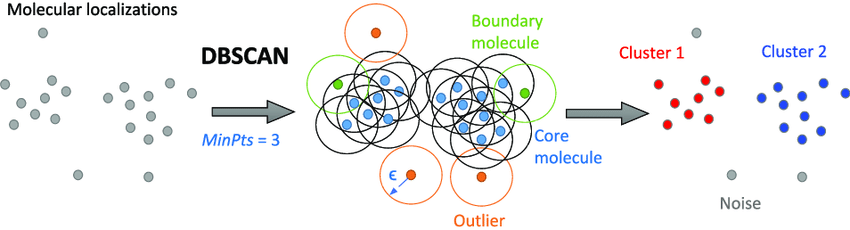
\includegraphics[width=0.9\linewidth]{png/An-Example-Illustrating-the-Density-Based-DBSCAN-Clustering-Method-Applied-to-SMLM-Data.png}
    \caption{An Example Illustrating the Density-Based DBSCAN Clustering Method Applied to SMLM Data}
    \label{fig:enter-label}
\end{figure}
Возникает 2 параметра: $\varepsilon$ и $m$. Других параметров не будет. От этих параметров и будет зависеть то, какой картина кластеризации получится. Также к преимуществам этого метода относится то, что он не задает заранее количество кластеров, в отличие, например, от k-means, причём количество кластеров будет зависеть от $\varepsilon$ и $m$. 

Как работает алгоритм: берётся произвольная точка, если она имеет плотную окрестность, то дальше рассматривается каждая точка этой плотной окрестности, и вокруг неё также строится $\varepsilon$-окрестность, и так пока не будет достигнута граница некоторого множества объектов. 

Хорошей аналогией может служить лес: один лес - это один кластер, через опушку, второй лес, - другой кластер, мы находимся в лесу. Смотрим, в нашей окрестности деревьев много, это значит, что мы в корневой точке находимся, и дальше мы идём, пока не выйдем на опушку леса, там мы окажемся в граничной точке - она уже не корневая, вокруг деревьев меньше. А где-то могут расти отдельно стоящие деревья - это шумовые выбросы. И вот так ходим по лесу, пока его весь не обойдём, и как только мы обошли весь лес, назовем его кластером. После чего случайно выбираем новое дерево и начинаем строить другой кластер.

Формализуем алгоритм в виде псевдокода:\\
\begin{tabularx}{\linewidth}{lX}
\textbf{вход:} выборка $X^l - \{x_1,...,x_l\}$; параметры $\varepsilon$ и $m$\\
\textbf{выход:} разбиение выборки на кластеры и шумовые выбросы;\\\hspace*{7mm}\hspace*{9mm}$U := X^l$ - не помеченные точки, $a := 0$\\
\textbf{пока} в выборке есть непомеченные точки, $U \neq \emptyset$:\\
\hspace*{7mm} взять случайную точку $x \in U$; \\
\hspace*{7mm} \textbf{если} $\abs{U_\varepsilon (x)} < m$ \textbf{то} \\
\hspace*{7mm}\hspace*{7mm} пометить $x$ как, возможно, шумовой;\\
\hspace*{7mm}\textbf{иначе} \\
\hspace*{7mm}\hspace*{7mm} создать новый кластер: $K:=U_\varepsilon (x); \; a:=a+1;$ \\
\hspace*{7mm}\hspace*{7mm} \textbf{для всех} $x' \in K$, не помеченных или шумовых \\
\hspace*{7mm}\hspace*{7mm}\hspace*{7mm} \textbf{если} $\abs{U_\varepsilon (x')} \geq m$,  \textbf{то} $K := K \cup U_\varepsilon (x')$; \\
\hspace*{7mm}\hspace*{7mm}\hspace*{7mm} \textbf{иначе} поментить $x'$ как граничный кластера $K$;\\
\hspace*{7mm}\hspace*{7mm} $a_j := a$ для всех $x_i \in K$;\\
\hspace*{7mm}\hspace*{7mm} $U := U \textbackslash K$;\\
\vspace{5mm}
\end{tabularx}

В таком виде алгоритм обладает следующими \textbf{свойствами}:
\begin{itemize}
    \item быстрая кластеризация больших данных: \\$O(l^2)$ в худшем случае, \\ $O(l \mathrm{ln} l)$ при эффективной реализации $U_\varepsilon (x)$;
    \item кластеры произвольной формы
    \item деление объектов на корневые, граничные, шумовые.
\end{itemize}

При этом важно понимать, что граничные объекты не выстраивают в точности границу каждого кластера. Практически это означает, что не стоит всерьез рассматривать граничные объекты, в отличие от шумовых, которые действительно можно в дальнейшем анализировать.

\subsection{Примечание о HDBSCAN} 
От гиперпараметра $\varepsilon$ можно избавиться, используя дивизивную кластеризацию. Такая модификация называется HDBSCAN. Его суть проста: необходимо построить дендрограмму, где по $Оу$ будет отложен $\varepsilon$ (на рис.\ref{fig:hdbdendro} снизу distance). Так мы сможем явно видеть вложенные кластеры. Алгоритм затем сам вычисляет оптимальное количество кластеров на основе метрики "стабильности кластеров".

\begin{figure}[h!]
    \centering
    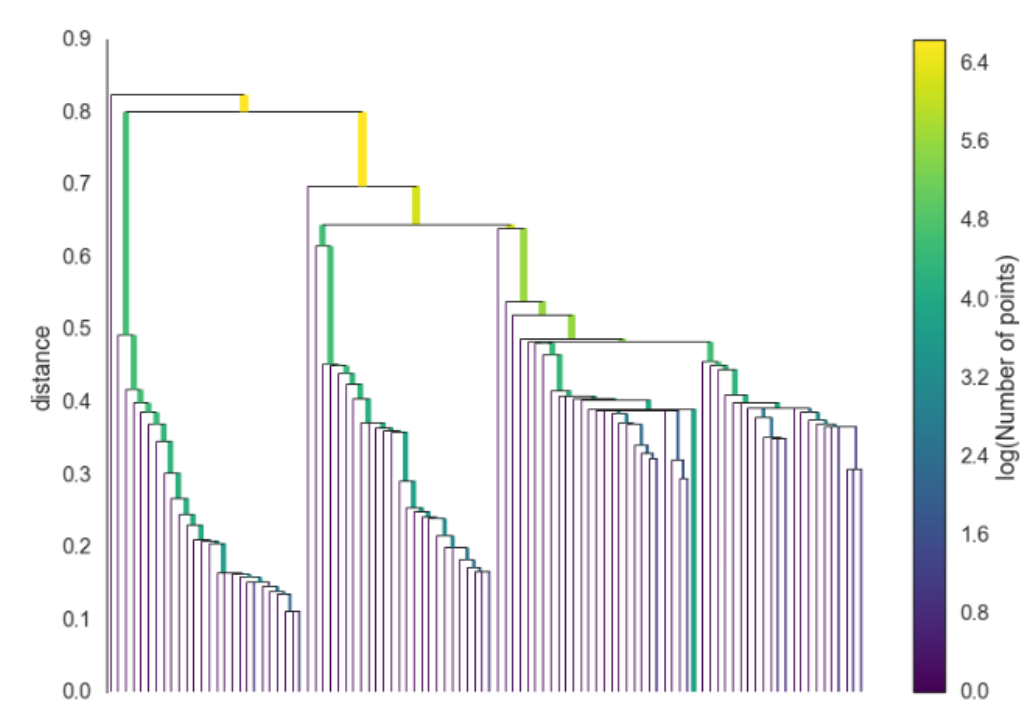
\includegraphics[width=0.6\linewidth]{png/hdbscan_dendrogramm.png}
    \caption{К примечанию о HDBSCAN}
    \label{fig:hdbdendro}
\end{figure}
\subsection{Задачи}
\textbf{Задача 1.}

\textbf{Условие.} Применить DBSCAN для выборки из таблицы с $m=4,\;\varepsilon=1.9$. Метрика евклидова.

\begin{center}
\begin{tabular}{ |c|c|c| } 
 \hline
 P1(3,7) & P5(7,3) & P9(3,3) \\ 
 P2(4,6) & P6(6,2) & P10(2,6) \\ 
 P3(5,5) & P7(7,2) & P11(3,5) \\ 
 P4(6,4) & P8(8,4) & P12(2,4) \\ 
 \hline
\end{tabular}
\end{center}

\textbf{Решение.}
Запишем матрицу, составленную из соответственных расстояний между точками выборки:
\begin{center}
\begin{tabular}{ |c|c|c|c|c|c|c|c|c|c|c|c|c|} 
 \hline
dot & P1 & P2 & P3 & P4 & P5 & P6 & P7 & P8 & P9 & P10 & P11 & P12 \\ \hline
P1 & 0 &  &  &  &  &  &  &  &  &  &  &   \\ \hline
P2 & 1.41 & 0 &  &  &  &  &  &  &  &  &  &   \\ \hline
P3 & 2.83 & 1.41 & 0 &  &  &  &  &  &  &  &  &   \\ \hline
P4 & 4.24 & 2.83 & 1.41 & 0 &  &  &  &  &  &  &  &   \\ \hline
P5 & 5.66 & 4.24 & 2.83 & 1.41 & 0 &  &  &  &  &  &  &   \\ \hline
P6 & 5.83 & 4.47 & 3.16 & 2.00 & 1.41 & 0 &  &  &  &  &  &   \\ \hline
P7 & 6.40 & 5.00 & 3.61 & 2.24 & 1.00 & 1.00 & 0 &  &  &  &  &   \\ \hline
P8 & 5.83 & 4.47 & 3.16 & 2.00 & 1.41 & 2.83 & 2.24 & 0 &  &  &  &   \\ \hline
P9 & 4.00 & 3.16 & 2.83 & 3.16 & 4.00 & 3.16 & 4.12 & 5.10 & 0 &  &  &   \\ \hline
P10& 1.41 & 2.00 & 3.16 & 4.47 & 5.83 & 5.83 & 5.66 & 6.40 & 6.32 & 0 &  &   \\ \hline
P11& 2.00 & 1.41 & 2.00 & 3.16 & 4.47 & 4.24 & 5.00 & 5.10 & 2.00 & 1.41 & 0 &   \\ \hline
P12& 2.83 & 3.16 & 4.00 & 5.10 & 4.47 & 5.39 & 6.00 & 1.41 & 2.00 & 2.00 & 1.41 & 0  \\ \hline
\end{tabular}
\end{center}
Сравнивая значения в каждом столбце матрицы с $\varepsilon$ и отбирая те, что меньше этого значения, находим окрестности каждой точки.

\begin{center}
\begin{tabular}{ |c|c| } 
 \hline
 точка & окрестность \\\hline
 P1 & P2, P10\\ 
 P2 & P1, P3, P11\\ 
 P3 & P2, P4\\ 
 P4 & P3, P5\\
 P5 & P4, P6, P7, P8\\
 P6 & P5, P7\\
 P7 & P5, P6\\
 P8 & P5\\
 P9 & P12\\
 P10 & P1, P11\\
 P11 & P2, P10, P12\\
 P12 & P9, P11\\
 \hline
\end{tabular}
\end{center}

Если в окрестности больше $m=4$ точек (включая ее саму), то отнесем эту точку к корневой, иначе - к шумовой.

\begin{center}
\begin{tabular}{ |c|c| } 
 \hline
 точка & тип \\\hline
 P1 & шум\\ 
 P2 & корневая\\ 
 P3 & шум\\ 
 P4 & шум\\
 P5 & корневая\\
 P6 & шум\\
 P7 & шум\\
 P8 & шум\\
 P9 & шум\\
 P10 & шум\\
 P11 & корневая\\
 P12 & шум\\
 \hline
\end{tabular}
\end{center}

Уточним классификацию, учтя граничные точки, т.е. точки, лежащие в окрестности корневых, но при этом не являющимися корневыми:
\begin{center}
\begin{tabular}{ |c|c| } 
 \hline
 точка & тип \\\hline
 P1 & граничная\\ 
 P2 & корневая\\ 
 P3 & граничная\\ 
 P4 & граничная\\
 P5 & корневая\\
 P6 & граничная\\
 P7 & граничная\\
 P8 & граничная\\
 P9 & шум\\
 P10 & граничная\\
 P11 & корневая\\
 P12 & граничная\\
 \hline
\end{tabular}
\end{center}

К первому кластеру отнесем окрестность корневой точки 2, причем в ее окрестности находится еще одна корневая точка 11, так что отнесем и ее окрестность к первому кластеру. Ко второму кластеру отнесем корневую точку 5 и ее окрестность. Осталась лишь одна точка P9, которая не относится ни к какому кластеру и является шумовой.
\begin{figure}[h!]
    \centering
    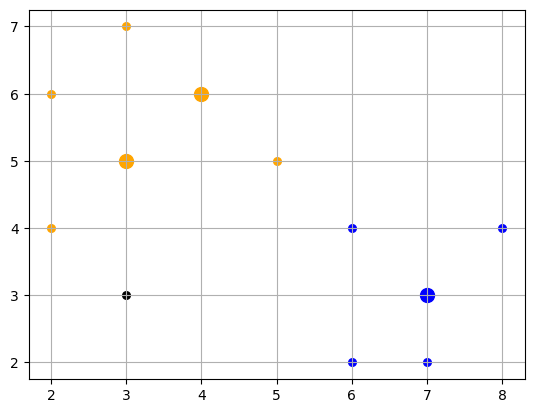
\includegraphics[width=0.7\linewidth]{png/task1dbs_plot.png}
    \caption{Кластеризация в задаче 1}
    \label{fig:task1dbs}
\end{figure}

\begin{minipage}{.5\textwidth}
\textbf{Задача 2.}\\
\textbf{Условие.}
  Сравните результаты кластеризации с помощью k-means и с помощью DBSCAN и объясните их.\\
\textbf{Решение.}
Объяснение различий:
\begin{itemize}
\item \textit{Форма кластера}:
K-средние: стремится найти сферические или выпуклые кластеры. Предполагается, что кластеры изотропны (однородны во всех направлениях) и имеют схожий размер.
DBSCAN: может обнаруживать кластеры произвольной формы и размера. Не делает предположений о форме кластеров.
\item \textit{Обработка шума}:
K-средние: плохо справляется с шумом. Точки шума могут быть назначены кластерам, что может повлиять на центры кластеров.
DBSCAN: может идентифицировать и маркировать точки шума, которые не назначены ни одному кластеру.
\end{itemize}
\end{minipage}% This must go next to `\end{minipage}`
\begin{minipage}{.4\textwidth}
      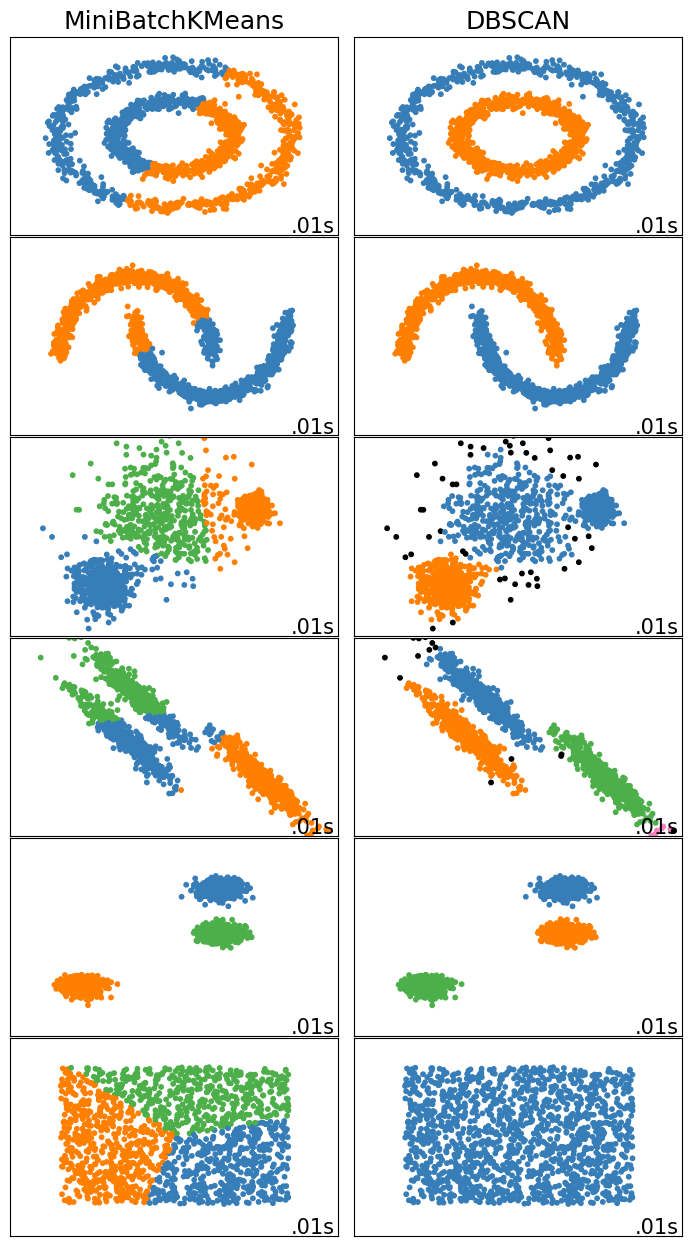
\includegraphics[width=0.95\linewidth]{png/task2dbs_plot.png}
\end{minipage}
\begin{itemize}
\item \textit{Плотность кластера}:
K-средние: не учитывает плотность точек. Каждый кластер представлен центроидом.
DBSCAN: учитывает плотность точек. Кластеры формируются на основе плотности точек в окрестности.
\item \textit{Чувствительность параметров}:
K-средние: требует предварительного указания количества кластеров (K), так что, если если заранее указать 3 кластера, то алгоритм и найдет три кластера, даже если он всего один, как на последней паре картинок.
\end{itemize}

\textbf{Задача 3.}\\
\textbf{Предисловие.}
При решении задачи 1 использовалась матрица, состоящая из расстояний между парами точек (\textit{матрица смежности}). Понятием, противоположным расстоянию, является понятие сходства между объектами. Неотрицательная вещественная функция $S(x_i,x_j) = S_{ij}$ называется \textit{мерой сходства}, если:
\begin{itemize}
    \item $0 \leq S(x_i,x_j) < 1$, для $x_i \neq x_j$
    \item $S(x_i,x_j)=1$
    \item $S(x_i,x_j)=S(x_j,x_i)$
\end{itemize}
Пары значений мер сходства можно объединить в \textit{матрицу сходства} $S$, симметричную и единичной диагональю.
\textbf{Условие.}
Применить DBSCAN с пороговым значением \textit{меры сходства} 0.8 и $m = 2$ и заданной матрицей сходства между точками выборки:

\begin{center}
\begin{tabular}{ |c|c|c|c|c|c|} 
 \hline
dot & P1 & P2 & P3 & P4 & P5  \\ \hline
P1 & 1.0 &  &  &  &     \\ \hline
P2 & 0.10 & 1.0 &  &  &  \\ \hline
P3 & 0.41 & 0.64& 1.0 &  & \\ \hline
P4 & 0.55 & 0.47 & 0.44 & 1.0 & \\ \hline
P5 & 0.35 & 0.98 & 0.85 & 0.76 & 1.0 \\ \hline
\end{tabular}
\end{center}

Сравнивая значения в каждом столбце матрицы с $\varepsilon$ и выбирая те точки, для которых значение сходства выше, чем порог, формируем окрестности всех точек.

\begin{center}
\begin{tabular}{ |c|c| } 
 \hline
 точка & окрестность \\\hline
 P1 & -\\ 
 P2 & P5\\ 
 P3 & P5\\ 
 P4 & -\\
 P5 & P2, P3\\
 \hline
\end{tabular}
\end{center}

Если в окрестности больше $m=2$ точек (включая ее саму), то отнесем эту точку к корневой, иначе - к шумовой.

\begin{center}
\begin{tabular}{ |c|c| } 
 \hline
 точка & тип \\\hline
 P1 & шум\\ 
 P2 & корневая\\ 
 P3 & корневая\\ 
 P4 & шум\\
 P5 & корневая\\
 \hline
\end{tabular}
\end{center}

Уточнение классификации, путем учитывания граничных точек, т.е. точек, лежащие в окрестности корневых, но при этом не являющимися корневыми, ничего не дает, т.к. в окрестности точек, определенных как шумовые вообще нет других точек, так что они действительно являются шумом.

К первому кластеру отнесем окрестность корневой точки P2, причем в ее окрестности находятся еще краевая точка P5, так что отнесем ее к этому же кластеру. В окрестности точки P5 помимо уже классифицированной P2 находится еще корневая точка P3, которую также отнесем к первому кластеру. Остальные точки классифицированы как шумовые. Таким образом в данной задаче всего один кластер, состоящий из точек P2, P3, P5.

\section{Простые эвристические методы частичного обучения}
\subsection{Постановка задачи}
Существует привычная нам задача классификации. Мы имеем $X$ --- множество объектов с известными признаками и $Y$ --- пространство классов. Есть неизвестная функция $X \longrightarrow Y$, сопоставляющая каждому обьекту его класс. Имеется обучающая выборка $\{x_1, x_2, ...\} \subset X$ и соответствующие им известные классы $\{y_1, y_2, ...\} \subset Y$. Задача классификации сводится к построению классификатора --- некой аппроксимации неизвестной функции $X \longrightarrow Y$. \\

С другой стороны существует задача кластеризации. Мы все также имеем $X$ --- множество объектов. И хотим аппроксимировать функцию $X \longrightarrow Y$. Но на этот раз у нас нет обучающей выборки, зато есть функция расстояния между объектами $\rho: X\times X \longrightarrow \mathbb{R}$. И в этом случае кластеризующая функция строится не на основе обучающей выборки, а так чтобы расстояние между объектами одного кластера было мало, а расстояние между объектами разных кластеров было велико. \\

Первый случай называется обучение с учителем,а кластеризация называется обучением без учителя. Где-то по середине между этими задачами находится задача частичного обучения. В этом случае у нас все также есть множество обьектов из $X$ и (возможно) функция $\rho$. При этом только для некоторой доли имеющихся обьектов известна классовая принадлежность. Иначе говоря обучающая выборка размечена \textbf{частично}. \\

Приведем пример (Рис. 1). Допустим известные обьекты в пространстве признаков имеют вид в виде двух бананов. И нам известна принадлежность только двух точек. В таком случае чистая задача кластеризации обучит классификатор только по двум точкам, который будет иметь сомнительное качество на всех остальных данных. При это частичное обучение могло бы учесть явную кластеризацию данных и дать значительно лучшую классификацию.\\

\begin{center}
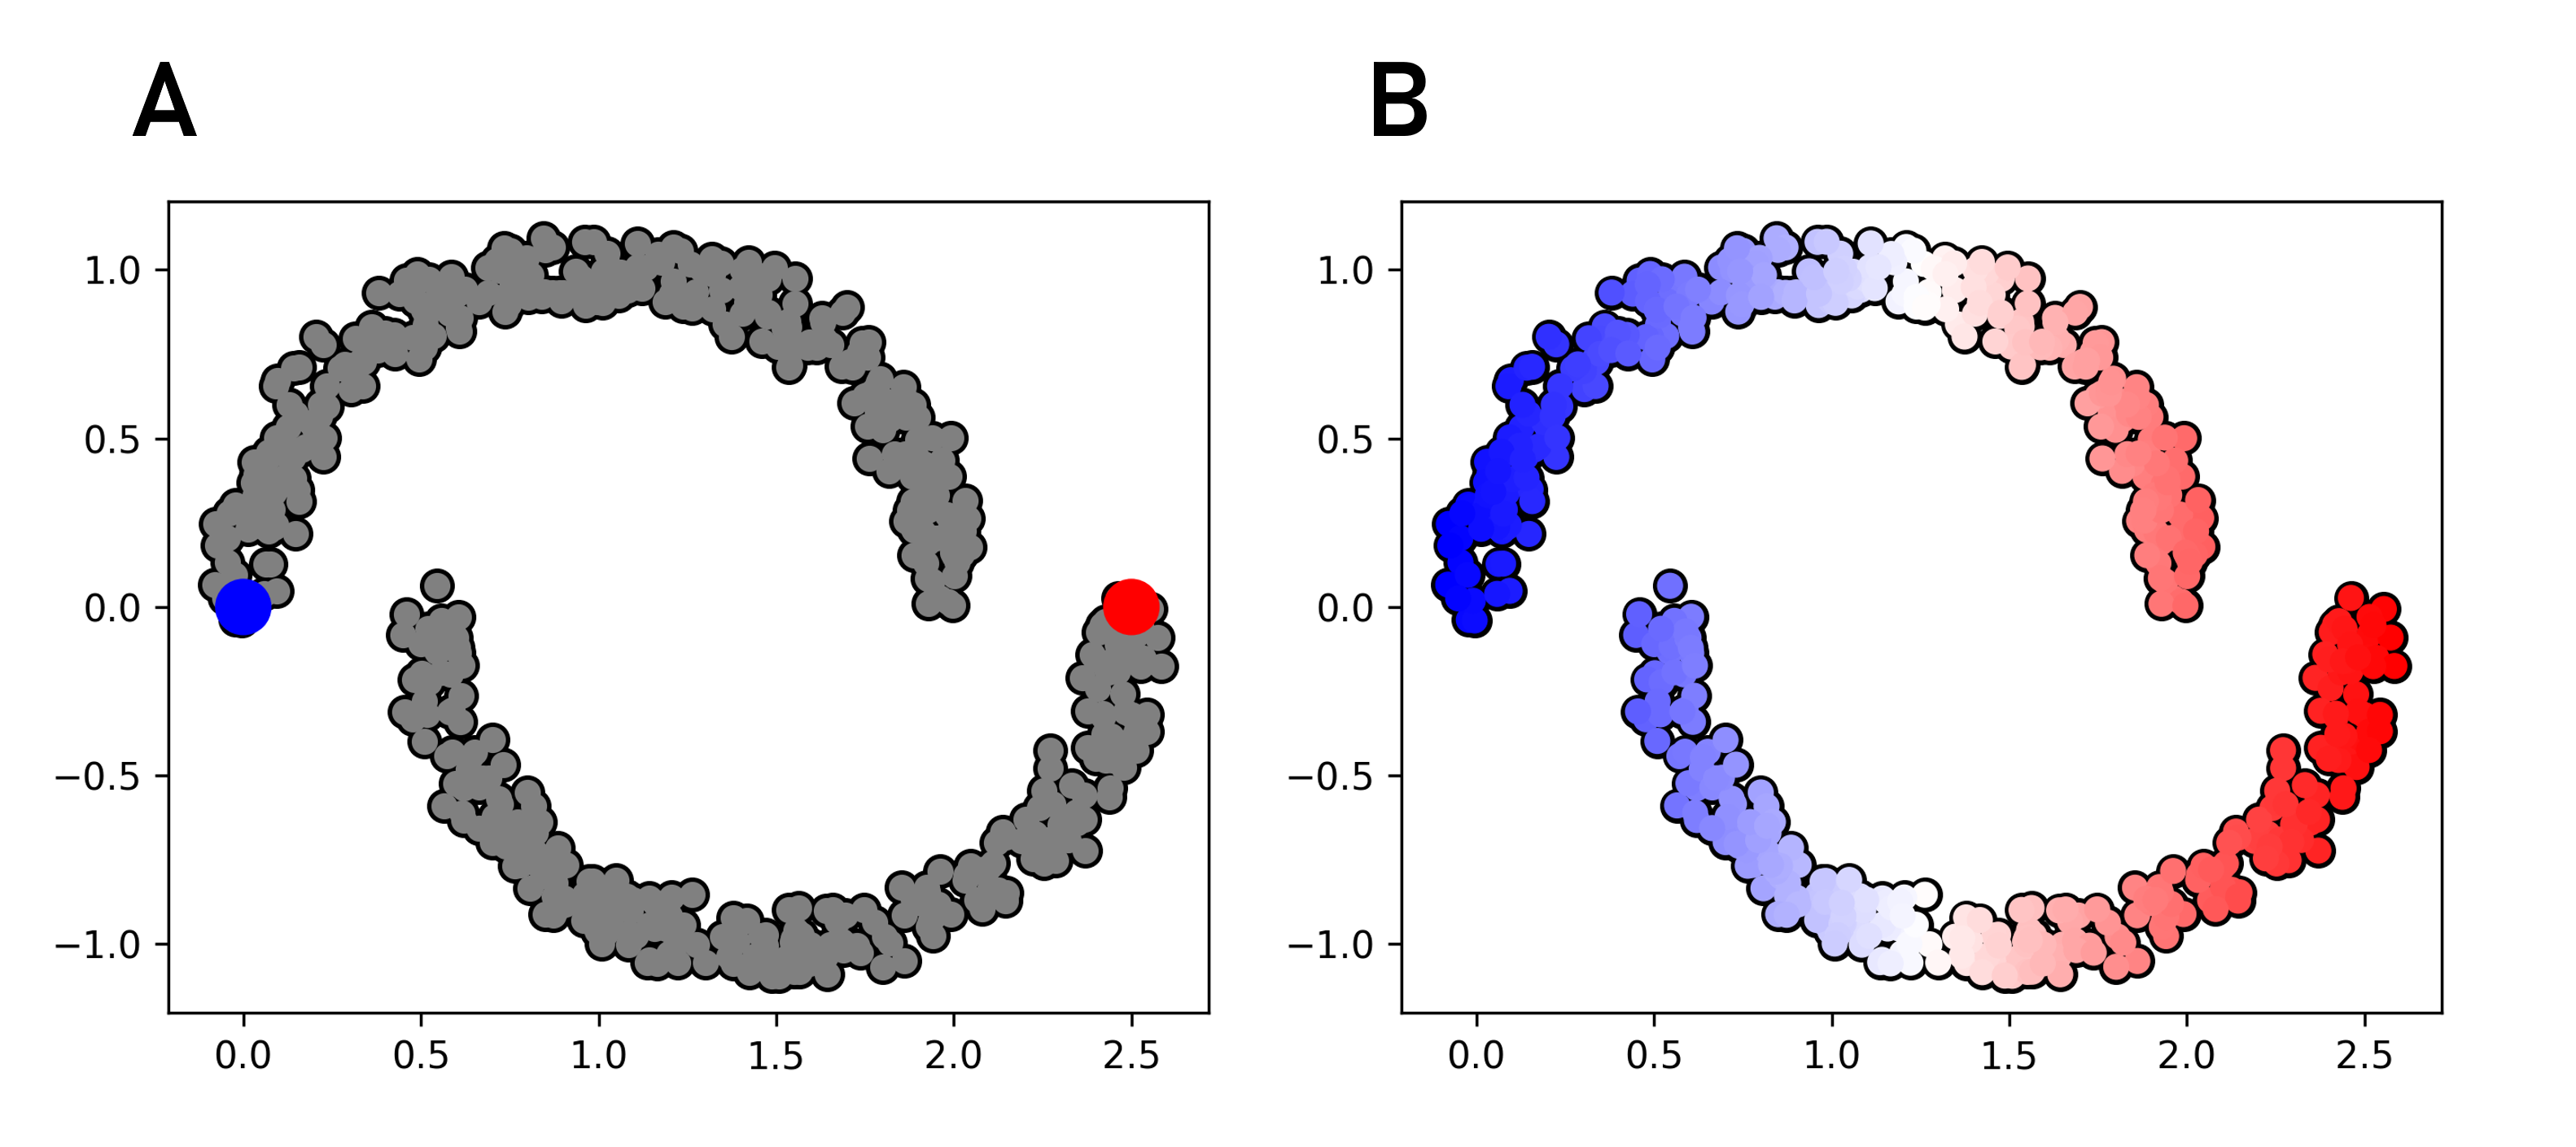
\includegraphics[width=1.0\textwidth]{picture_1.png}
\textbf{Рисунок 1.} (\textbf{A}) Пример частично размеченных данных. (\textbf{B}) Классификация обученная на размеченных данных не учитывает кластерную структуру неразмеченных. 
\end{center}

Однако частичное обучение не может сводиться только к кластеризации, представьте теперь, что мы знаем классы уже трех точек на выборке из двух бананов (Рис. 2). В таком случае кластеризация дала бы предсказание которое не может соотноситься с известными классами всех трех точек. Таким образом задача частичного обучения действительно находится посередине между классификацией и кластеризацией, но не является ни тем, ни другим. \\
\begin{center}
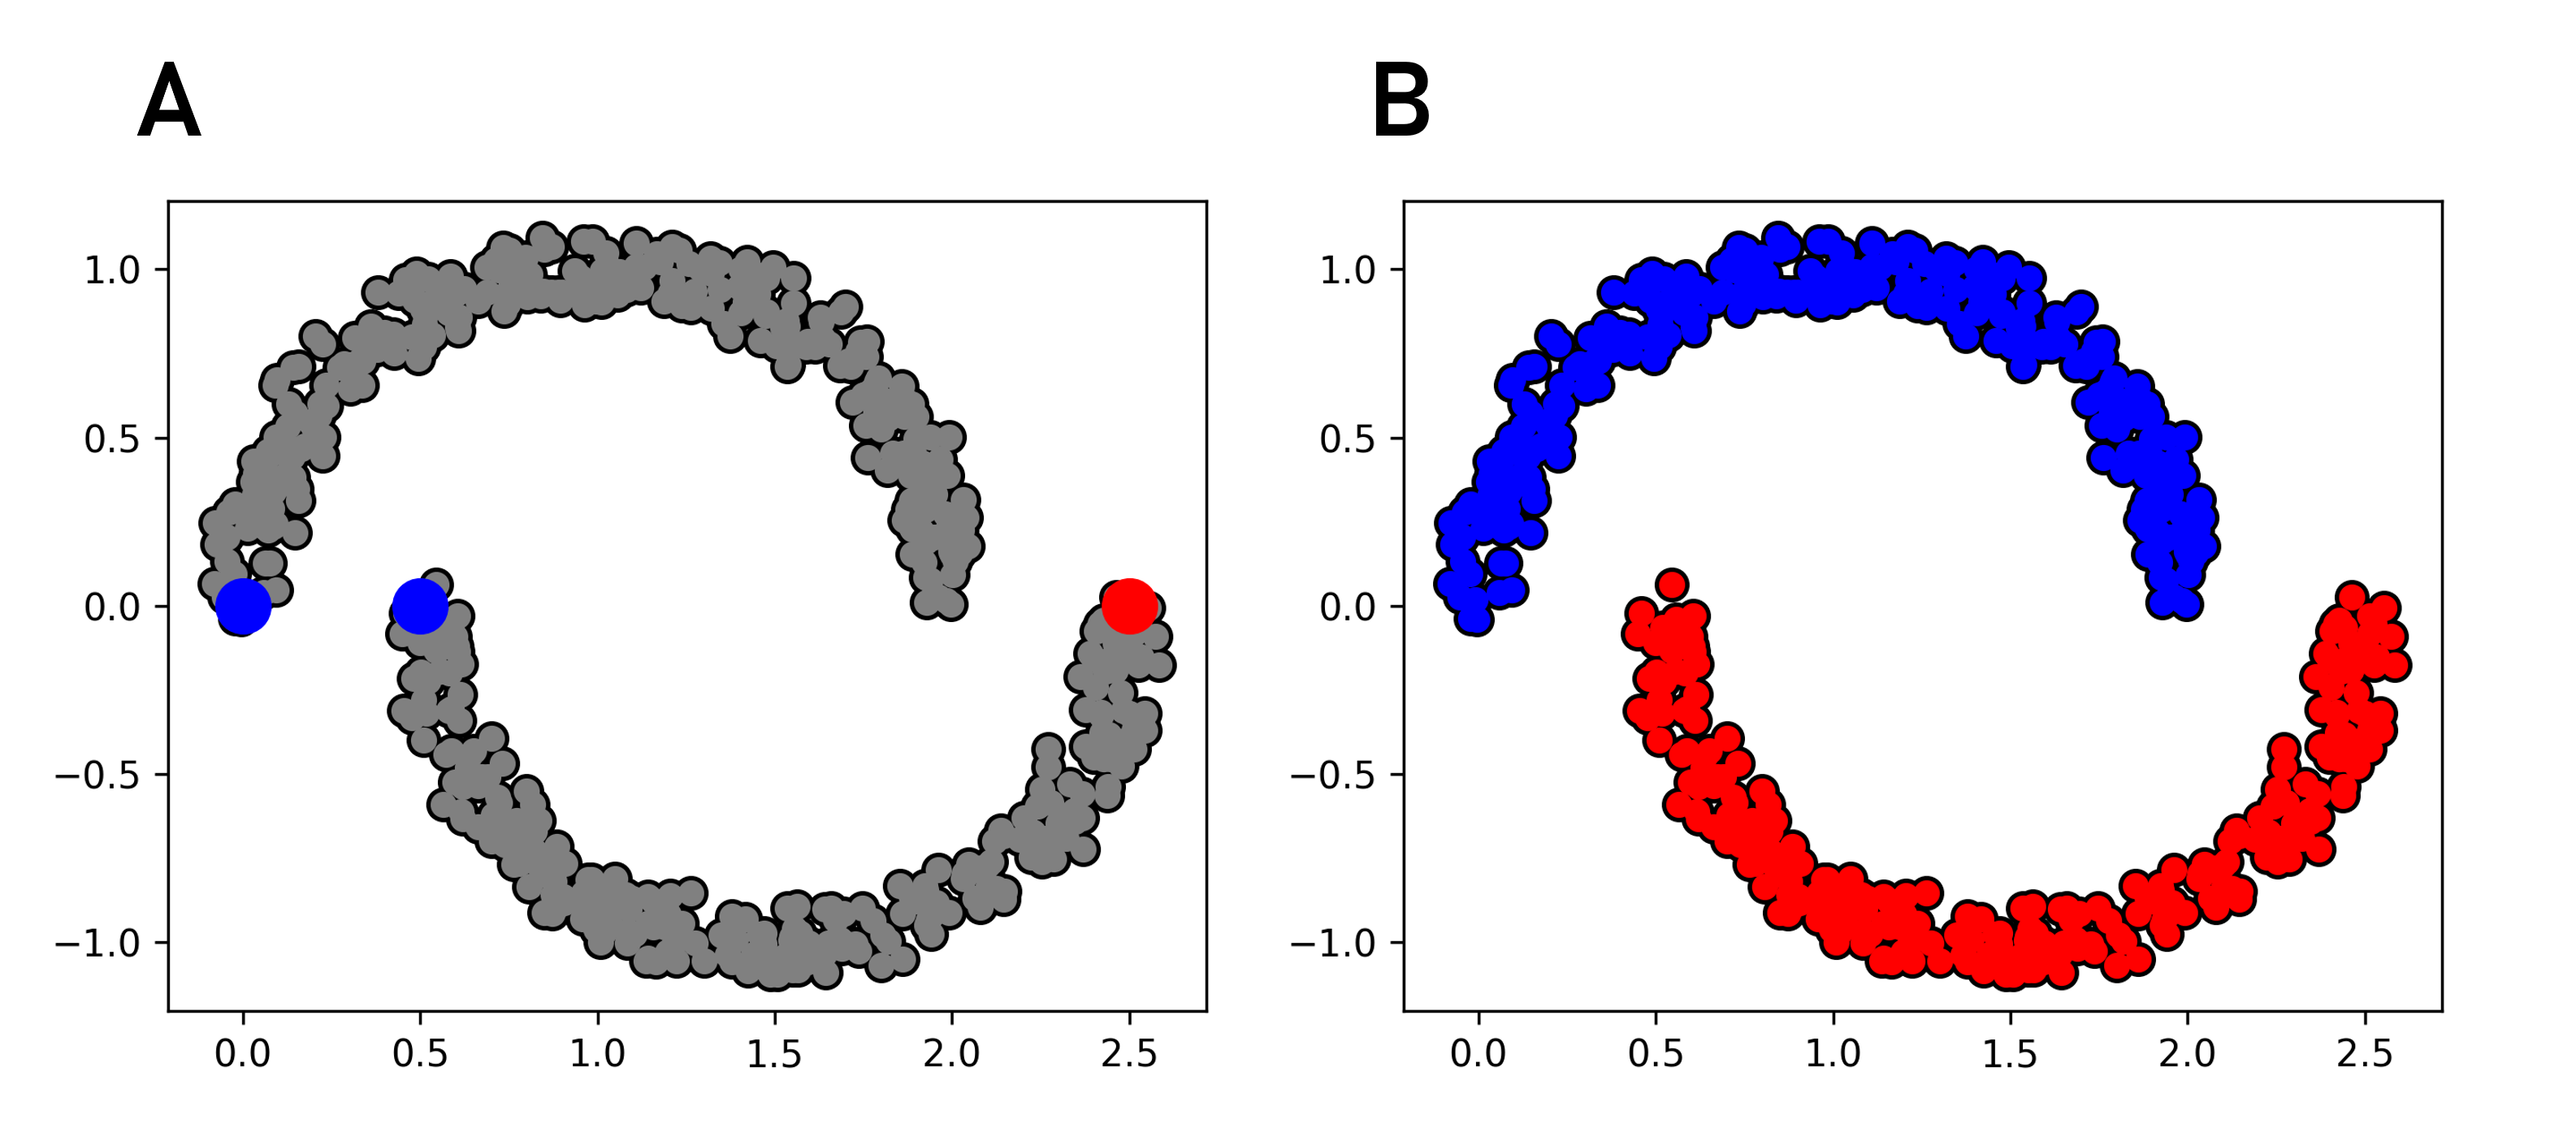
\includegraphics[width=1.0\textwidth]{picture_2.png}
\textbf{Рисунок 2.} (\textbf{A}) Пример частично размеченных данных. (\textbf{B}) Кластеризация не учитывает классовую принадлежность размеченных данных. 
\end{center}

Приведем пример: программист решил сделать классификатор для фотографий котиков и собачек, для этого он скачал по миллиону фотографий и тех и других. Однако, ему хватило сил подписать котик это или собачка только для 1000 фотографий. Классификация не может быть построена только по 1000 фотографиям --- мало данных, а кластеризация может разбить фотографии неизвестным образом --- по цвету фона, по размеру животного. И только частичное обучение может помочь ленивому программисту.
\subsection{Self-training}
Каким же образом можно реализовать частичное обучение? Рассмотрим подход, который называется self-training (само-обучение). Вернемся к датасету с бананами в котором известны классы двух точек. Как было сказано ранее построение классификатора по двум точкам тут не поможет. Однако допустим, что мы все же построили классификатор по двум точкам, к примеру логистическую регрессию. Вспомним что многие методы классификации могут оценивать свою уверенность в предсказании. Тогда для некоторых точек с наибольшей уверенностью классификации (скажем 5\% самых уверенных) предсказание  классификации может оказаться вполне верным. Давайте же дополним обучающую выборку классификатора этими точками. На второй итерации нашего подхода мы обучим классификатор уже по дополненной обучающей выборке. Выполнив предсказание для остальных данных, выберем еще раз 5\% ранее неразмеченных точек с наибольшей уверенностью и пополним ими обучающую выборку. Будем повторять такие итерации пока не классифицируем все точки в нашем датасета. Как мы видим, результат такого подхода заметно лучше, чем у классификации по двум исходным точкам. 
\begin{center}
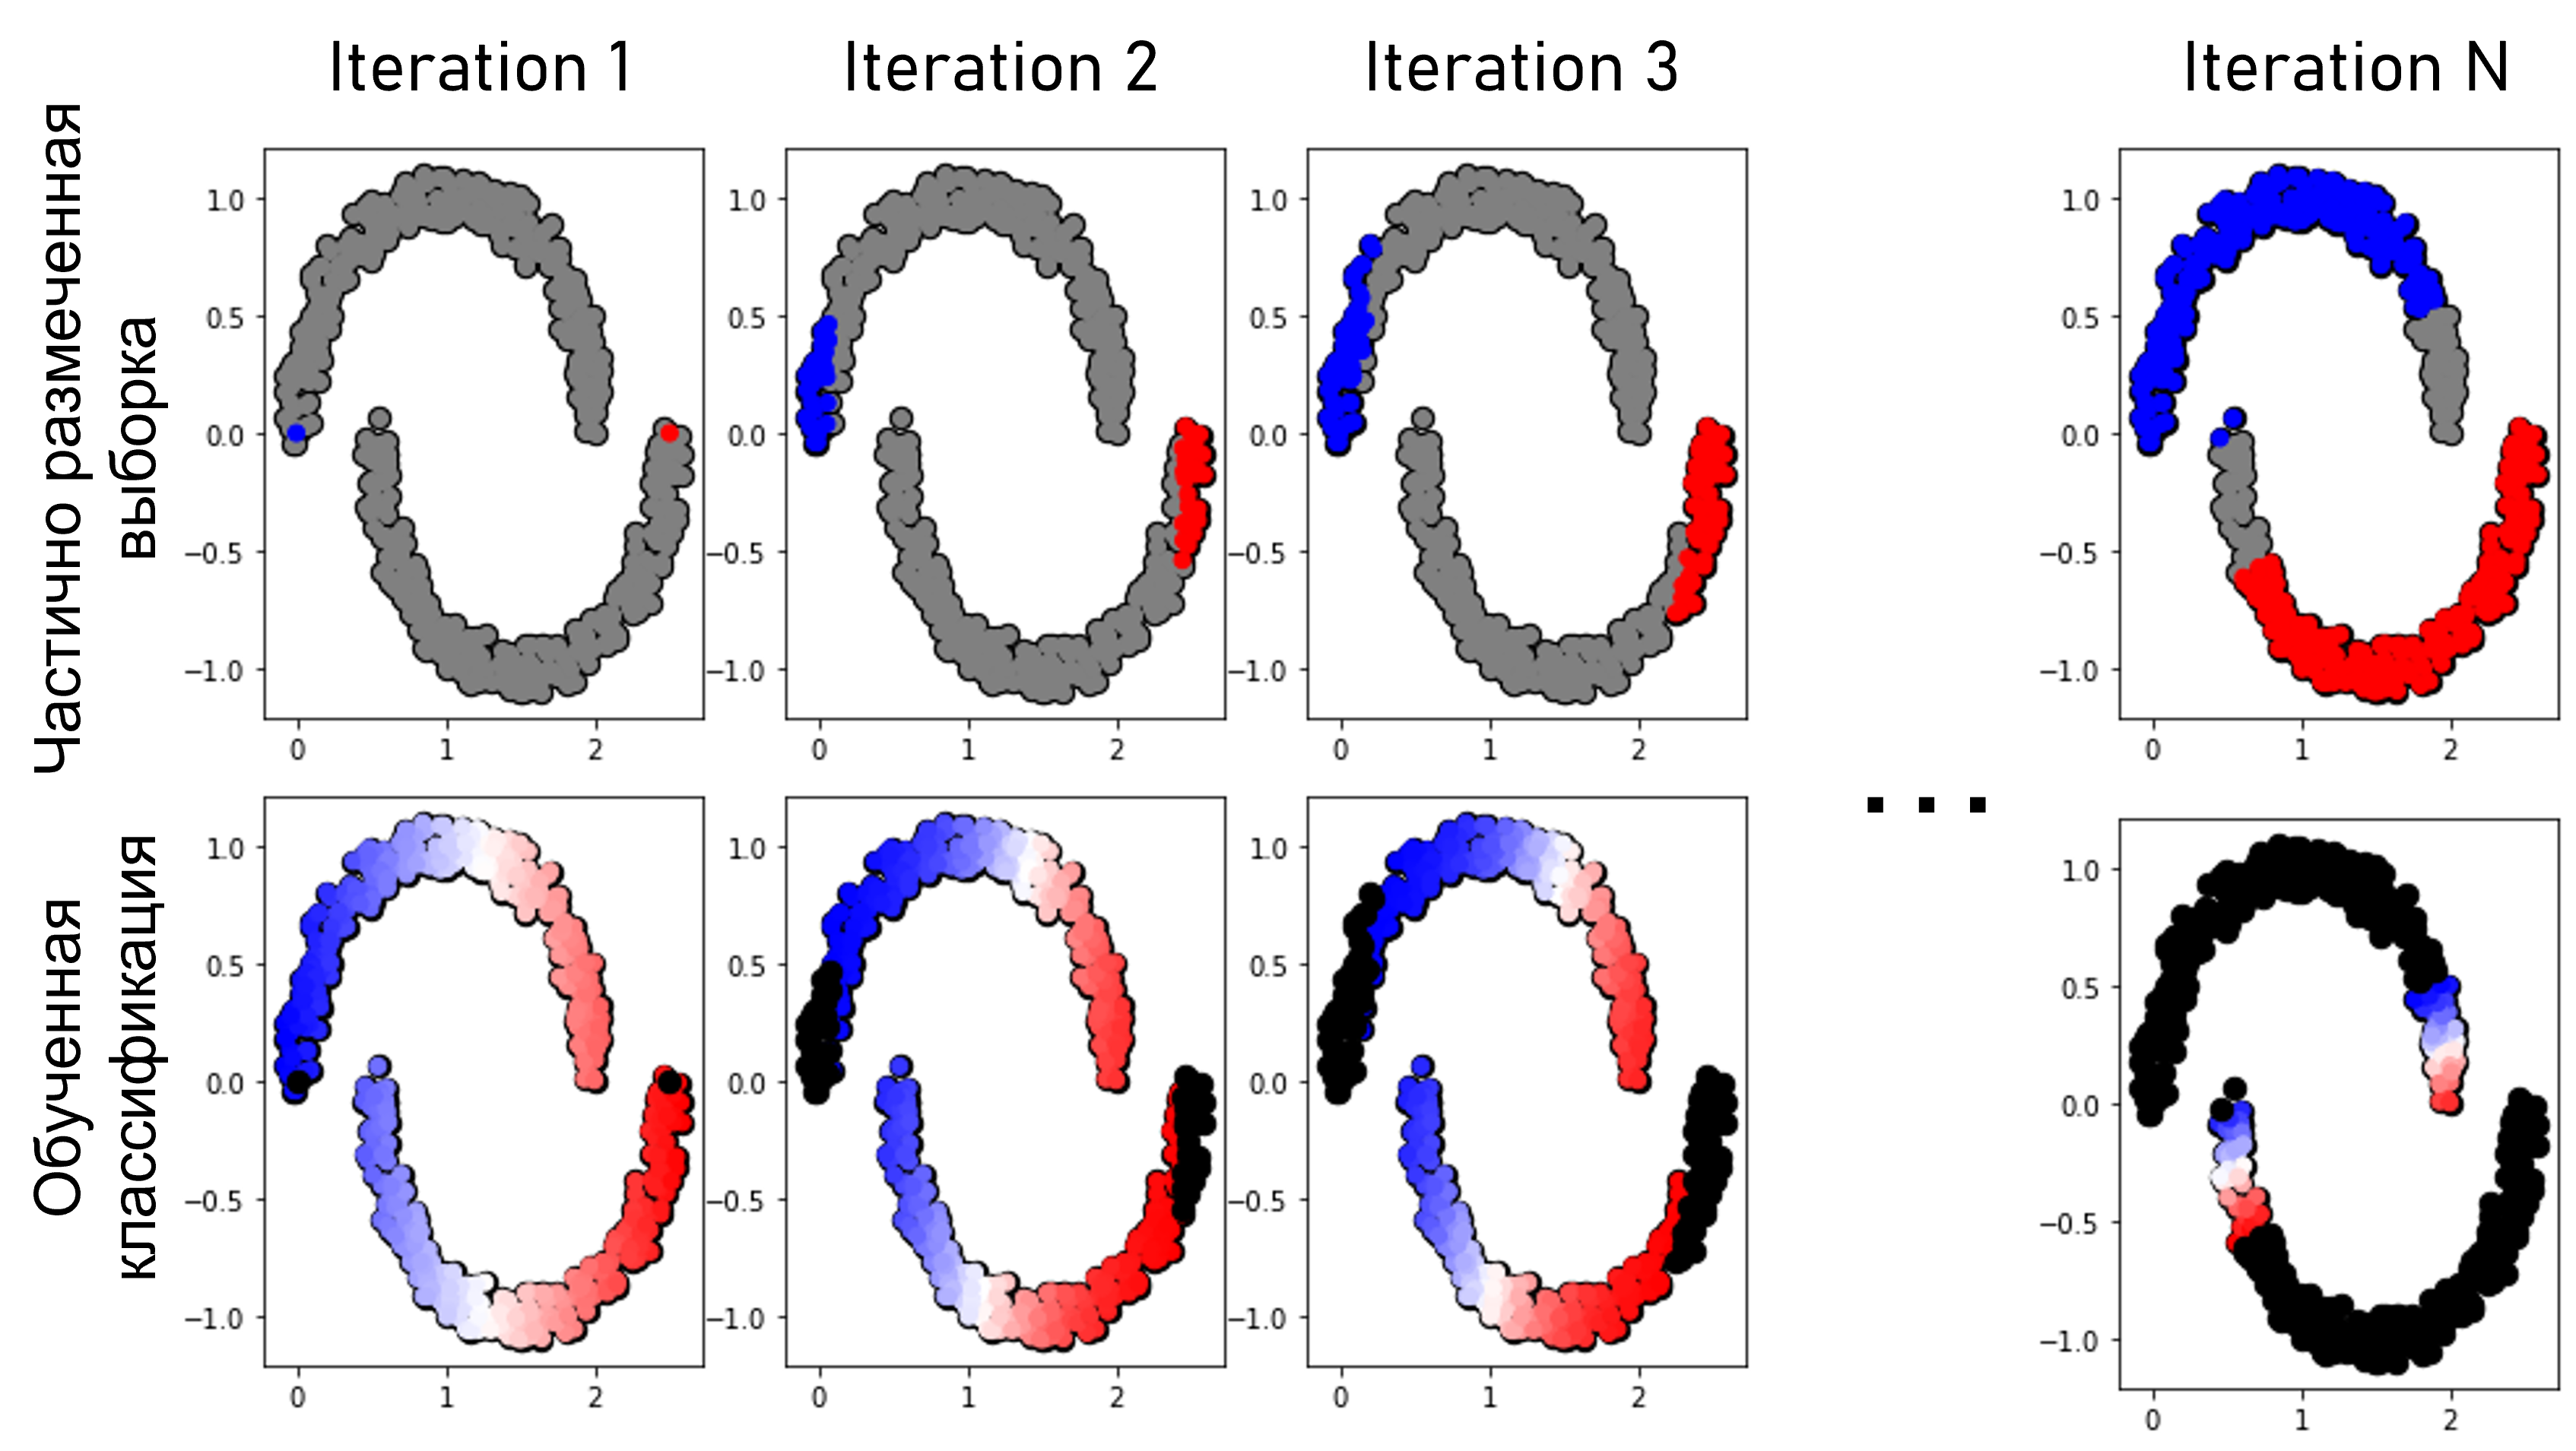
\includegraphics[width=1.0\textwidth]{picture_3.png}
\textbf{Рисунок 3.} Пример работы итераций self-training. 
\end{center}
Оформим описанный процесс более математизировано. Пусть мы строим функцию $a: X \longrightarrow Y$. Пусть у нас есть метод обучения функции $\mu: Z \longrightarrow a$ который принимает на вход размеченную часть выборки $Z \subset X$. Допустим функция $a$ имеет вид
\begin{equation*}
    a(x) = \arg \max_{y \subset Y}\Gamma_y(x)
\end{equation*}
где $\Gamma_y(x)$ это некоторые (к примеру) линейные функции от $x \subset X$ которые обучаются так, чтобы быть большими, если $x$ принадлежит классу $y$ и маленькими в противном случае. В таком случае уверенность классификации в принадлежности элемента $x$ к классу $y_1$ (отступ):
\begin{equation*}
    M_1(x) = \Gamma(x) - \max_{y \subset Y\backslash y_1}\Gamma_{y_1}(x) 
\end{equation*}
Пусть $Z$ это размеченная часть обучающей выборки. Тогда алгоритм выглядит так:
\begin{enumerate}
  \item $a = \mu(Z)$ --- обучить классификатор на размеченной выборке
  \item $\Delta := \{x \subset X\backslash Z \;|\; M(x) \geq M_0 \}$ --- выбрать несколько точек из неразмеченной части выборки которые наиболее уверенно классифицируются. 
  \item $Z := Z\cup\Delta$ --- дополнить размеченную выборку
  \item Если не все элементы выборки размечены, вернуться в начало.
\end{enumerate}
\subsection{Сo-training}
Рассмотрим более узкий кейс, допустим у нас есть не один, а целых два метода обучения классификации $\mu_1, \mu_2$, которые принципиально отличаются друг от друга, например имеют разные парадигмы обучения, и/или используют разные признаки обьектов, и/или имеют разную стартовую выборку. В таком случае мы можем получить преимущество в частичном обучении заставив их учить друг друга по следующему алгоритму:
\begin{enumerate}
  \item $a_1 = \mu_1(Z_1)$\\
  $a_2 = \mu_2(Z_2)$ --- два метода обучают классификаторы на своих размеченных выборках. 
  \item $\Delta_1 := \{x \subset X\backslash Z_1\backslash Z_2 \;|\; M_1(x) \geq M_{01} \}$ --- метод 1 размечает неразмеченные точки, в которых он уверен.\\
  $\Delta_2 := \{x \subset X\backslash Z_1\backslash Z_2 \;|\; M_2(x) \geq M_{02} \}$ --- метод 2 делает тоже самое.
  \item $Z_1 := Z_1\cup\Delta_2$ --- метод 2 дополняет обучающую выборку метода 1 \\
  $Z_2 := Z_2\cup\Delta_1$ --- метод 1 дополняет обучающую выборку метода 2
  \item Если не все элементы выборки размечены, вернуться в начало.
\end{enumerate}
\subsection{Сo-learning}
Идем еще дальше, допустим у нас теперь есть набор методов $\mu_i$ отличающиеся чем-то. Допустим что все эти методы обучились на одной выборке $Z$ и произвели классификаторы $a_i$. Давайте соберем из множества классификаторов $a_i$ один классификатор-мегазорд:
\begin{equation*}
    a(x) = \arg \max_{y \subset Y}\Gamma_y(x)
\end{equation*}
Где на этот раз функции $\Gamma$ определяются как:
\begin{equation*}
    \Gamma_y(x) = \sum_{i = 1}^{I}[a_i(x) = y]
\end{equation*}
Выражение в квадратных скобках равно 1 когда написанное в них верно, и равно 0 в противных случаях. Иначе говоря, классификаторы $a_i$ голосуют за принадлежность к классам, и демократически выбирают к кому классу отнести каждый из обьектов. Далее на основе такого обьединенного классификатора строится Self-training описанный выше. 
\subsection{Задачи}
\subsection*{Задача 1}
Возможно ли при помощи self-training эффективно классифицировать точки частично размеченной выборки представленной ниже:
\begin{center}
\includegraphics[width=0.5\textwidth]{picture_5.png}
\end{center}
\textit{\textbf{Решение:} Конечно можно! Для этого нужно построить self-training на основе классификатора который может делать разделяющую поверхность в виде окружности, например классификаторы восстанавливающие плотность или логистическая регрессия с добавлением квадратичных признаков}
\subsection*{Задача 2}
Два подхода частичного обучения применяются для классификации обьектов частичной выборки представленной ниже.
\begin{center}
\includegraphics[width=0.5\textwidth]{picture_4.png}
\end{center}
Первый подход это self-training на основе логичтической регрессии, которая видит только первый признак. Второй подход это co-training на основе двух логистических регрессий, таких что первая видит первый признак, а вторая второй. Какой алгоритм приведет к лучшей классификации точек и почему?\\

\textit{\textbf{Решение:} self-training видящий только первый признак веротянее всего идеально классифицирует точки, так как по этому признаку кластеры разделены и практически не пересекаются. В случае co-training классификатор использующий второй признак видит кластеры пересекающимися и почти наверняка наделает ошибок при классификации}
\subsection*{Задача 3}
Алгоритм co-training построенный на основе трех классификаторов классифицирует точки представленной ниже выборки. На последней итерации работы алгоритма осталась лишь одна неклассифицированная точка. На этот момент классификаторы имеют разделяющие линии представленные на картинке. К какому кластеру будет отнесена оставшаяся точка?
\begin{center}
\includegraphics[width=0.5\textwidth]{picture_6.png}
\end{center}
\textit{\textbf{Решение:} Судя по разделяющим линиям два классификатора проголосую за красный кластер, и только один за синий, в итоге точка будет отнесена к красному кластеру.}

\subsection*{Алгоритм Ланса-Уильямса} % Aleksandrov Nikta

Пусть $X = \{\{x_1\},..., \{x_l\}\}$ - исходная выборка, $l$ - количество её элементов, необходимо объединить объекты выборки в кластере на основе расстояний между ними. Алгоритм инициализируется таким образом, что каждый объект выборки считается отдельным кластером, затем происходит итеративное слияние кластеров друг с другом. Критерием, по которому кластеры объединяются, является расстояние между ними. %$R(\{x_i\}, \{x_j\}) = \rho (x_i, x_j)$.
Существует множество способов выбора метрики расстояния между кластерами, однако большинство классических метрик можно обобщить, используя формулу Ланса-Уильямса.\\
Пусть в процессе вычисления имеется набор кластеров $C_t,t \in \{1, \l\}$, $U, V$ - кластеры, которые были выбраны для слияния, $W = U \cup V$ , тогда для произвольного кластера $S \in C_t\ \cup \{W\} \textbackslash \{U, V\}$ расстояние $R_{WS}$ до кластера $W$ определяется по следующей формуле.

\begin{equation*}
        R_{WS} = \alpha_U \cdot R_{US} + \alpha_V \cdot R_{VS} + \beta \cdot R_{UV} + \gamma \cdot |R_{US} - R_{VS}|
\end{equation*}

где $R_{US}, R_{VS}, R_{UV}$ - расстояния между кластерами $U$ и $S$, $V$ и $S$, $U$ и $V$ соответственно, $\alpha_U, \alpha_V, \beta, \gamma$ - некоторые действительные коэффициенты. Рассмотрим стандартные способы задания метрики расстояния между множествами и покажем, какие значения коэффициентов соответствуют им:

\begin{itemize}
    \item Расстояние до ближайшего соседа: $R^{\text{б}}_{WS} = \underset{w \in W, s \in S}{min}
  \rho (w, s)$; $\alpha_U = \alpha_V = \frac{1}{2}, \beta = 0, \gamma = - \frac{1}{2}$
    \item Расстояние до наиболее удалённого соседа: $R^{\text{д}}_{WS} = \underset{w \in W, s \in S}{max} \rho (w, s)$; $\alpha_U = \alpha_V = \frac{1}{2}, \beta = 0, \gamma = \frac{1}{2}$
    \item Среднее расстояние между элементами кластера: $R^{\text {с}}_{WS} = \frac{1}{|W||S|} \sum_{w \in W} \sum_{s \in S} \rho (w, s)$; $\alpha_U = \frac{|U|}{|W|}, \alpha_V = \frac{|V|}{|W|}, \beta = \gamma = 0$
    \item Расстояние между центрами: $R^{\text{ц}}_{WS} = \rho^2 \left( \sum_{w \in W} \frac{w}{|W|}, \sum_{s \in S} \frac{s}{|S|} \right)$; $\alpha_U = \frac{|U|}{|W|}, \alpha_V = \frac{|V|}{|W|}, \beta = \alpha_U \cdot \alpha_V, \gamma = 0$
    \item Расстояние Уорда: $R^{\text{у}}_{WS} = \frac{|S||W|}{|S|+|W|} \rho^2 \left( \sum_{w \in W} \frac{w}{|W|}, \sum_{s \in S} \frac{s}{|S|} \right)$; $\alpha_U = \frac{|S| + |U|}{|S|+|W|}, \alpha_V = \frac{|S|+|V|}{|S|+|W|}, \beta = \frac{-|S|}{|S|+|W|}, \gamma = 0$
\end{itemize}

Таким образом, данная метрика действительно является обобщением множества классических способов определения расстояния между кластерами. Ниже представлен псевдокод алгоритма Ланса-Уильямса.

\begin{algorithm}
\caption{Агломеративная кластеризация Ланса-Уильямса}\label{Lance–Williams}
\begin{algorithmic}
\State $t:=1$: $C_t = \{\{x_1\},...,\{x_l\}\}$
\ForEach {$s \in \mathcal S $}
\State найти в $C_{t - 1}$ пару кластеров $U, V$ с минимальным $R_{UV}$
\State $W = U \cup V;$
\State $C_t = C_{t - 1} \cup \{W\} \textbackslash \{U, V\};$
\ForEach {$S \in C_t$}
\State $R_{WS} = \alpha_U \cdot R_{US} + \alpha_V \cdot R_{VS} + \beta \cdot R_{UV} + \gamma \cdot |R_{US} - R_{VS}|$

\end{algorithmic}
\end{algorithm}

На выходе алгоритма получается кластер, состоящий из всех элементов исходной выборки, разделённый иерархически на подкластеры. Дальнейшей задачей является выделение основных подкластеров из данного набора кластеров для дальнейшей работы с ними. Это удобно сделать, используя дендрограмму - график, визуализирующий расстояние между кластерами, образующимися в процессе вычислений.

\begin{center}
\begin{figure}[H]
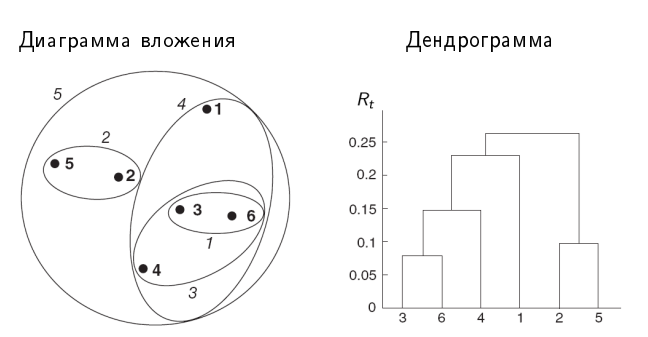
\includegraphics[width=14cm]{Dendrogramma.png}
\caption{Визуализация объектов кластеров и соответствующая им дендрограмма для алгоритма Ланса-Уильямса, в качестве расстояния используется расстояние Уорда}
\label{fig:Dendrogramma}
\end{figure}
\end{center}

На данной дендрограмме можно провести горизонтальную линию по уровню $R_0$, что и определит конечную структуру кластеров. Проще всего сделать это путём отсечения правого участка дендрограммы. На горизонтальной оси находится интервал максимальной длины $|R_{t+1} - R_t|$, в качестве результирующей кластеризации выдаётся множество кластеров $C_t$, их число $K = l - t + 1$. Для того, чтобы улучшить качество кластеризации, необходимо, чтобы метрика расстояния обладала определёнными свойствами.

\subsection*{Монотонность}

Функция расстояния $R$ обладает свойством монотонности, если при каждом слиянии расстояние между объединяемыми кластерами увеличивается: $R_2 \leq R_3 \leq...\leq R_l$. В таких случая дендрограмму можно построить без самопересечений, что в свою очередь позволяет выделить чёткую кластерную структуру. Существует достаточное условие монотонности функции расстояния:

\textbf{Теорема Миллигана.} Если выполняются следующие 3 условия, то кластеризация является монотонной
\begin{itemize}
    \item $\alpha_U \geq 0, \alpha_V \geq 0$;
    \item $\alpha_U + \alpha_V + \beta \geq 1;$
    \item $min \{{\alpha_U, \alpha_V}\} + \gamma \geq 0$
\end{itemize}

\subsection{Свойства растяжения и сжатия}

Фукнция расстояния $R$ обладает свойством растяжения, если при каждом слиянии расстояние от него до других кластеров увеличивается. Функция расстояния $R$ обладает свойством сжатия, если при каждом слиянии расстояние от него до других кластеров уменьшается. Растяжение способствует более чёткому отделению кластеров, однако при избыточно слишком большом растяжении некоторые кластеры находятся там, где их изначально не было. На практике используется гибкое расстояние, являющееся компромиссом между методами ближнего, дальнего соседа и среднего расстояния, регуляруется параметром $\beta$: $\alpha_U = \alpha_V = (1 - \beta)/2, \beta < 1$. При $\beta > 0$ расстояние является сжимающим, при $\beta < 0$ растягивающим. Более точный подбор $\beta$ проводится на основе анализа конкретной задачи. 

В целом, нельзя однозначно сказать, какой выбор коэффициентов даст лучший результат. Среди перечисленных расстояний наиболее стабильным принято считать расстояние Уорда. Однако для улучшения качества кластеризации рекомендуется исследовать алгоритм на точность при различных вариантах метрики. 

\subsection*{Задачи на данную тему}

\subsubsection*{Задача 1} 
Сгенерируйте 2 двухмерых гауссиана с единичными матрицами ковариации, но различными векторами средних. Используйте алгоритм Ланса-Уильямса для кластеризации получившихся наборов точек. Проведите вычисления для разных значений $|\Vec{\mu_1} - \Vec{\mu_2}|$, где $\Vec{\mu_1}$ - вектор среднего для первого гауссиана, $\Vec{\mu_2}$ - вектор среднего для второго гауссиана. Сравните полученные результаты с результатами, получаемыми с помощью алгоритма восстановления плотности вероятности. 

\subsubsection*{Задача 2} 
Возьмите статистику по среднему баллу по базовым кафедральным предметам, количество времени, проводимого на кафедре и на работе/стажировке, а также зарплату для всех студентов вашего потока. Используйте алгоритм Ланса-Уильямса и оцените, насколько часто студенты одной кафедры оказываются в одном кластере. 

\subsubsection*{Задача 3} 
Возьмите данные о поведение акций Мосбиржи за последний месяц, для каждой акции определите такие показатели, как средняя цена, средняя прибыль, размер дивидентов (при выплате) и др., затем проведите кластеризацию. Какие выводы можно сделать на основании полученных данных? Можно ли определить, какие бумаги более предпочтительны для покупки.

\end{document}
